\documentclass[letterpaper,final,12pt,reqno]{amsart}

\usepackage[total={6.3in,9.2in},top=1.1in,left=1.1in]{geometry}

\usepackage{empheq}
\usepackage[dvipsnames]{xcolor}
\usepackage{graphicx}
\usepackage{fancyvrb}

%\usepackage{palatino}

% hyperref should be the last package we load
\usepackage[pdftex,
colorlinks=true,
plainpages=false, % only if colorlinks=true
linkcolor=blue,   % only if colorlinks=true
citecolor=Red,   % only if colorlinks=true
urlcolor=black     % only if colorlinks=true
]{hyperref}

\renewcommand{\baselinestretch}{1.05}

\newcommand{\ddt}[1]{\ensuremath{\frac{\partial #1}{\partial t}}}
\newcommand{\ddx}[1]{\ensuremath{\frac{\partial #1}{\partial x}}}
\newcommand{\ddy}[1]{\ensuremath{\frac{\partial #1}{\partial y}}}
\newcommand{\pp}[2]{\ensuremath{\frac{\partial #1}{\partial #2}}}
\renewcommand{\t}[1]{\texttt{#1}}
\newcommand{\Matlab}{\textsc{Matlab}\xspace}
\newcommand{\eps}{\epsilon}
\newcommand{\RR}{\mathbb{R}}

\newcommand{\grad}{\nabla}
\newcommand{\Div}{\nabla\cdot}
\newcommand{\trace}{\operatorname{tr}}


\newcommand{\hbn}{\hat{\mathbf{n}}}

\newcommand{\bg}{\mathbf{g}}
\newcommand{\bu}{\mathbf{u}}
\newcommand{\bv}{\mathbf{v}}

\newcommand{\bX}{\mathbf{X}}



\begin{document}
\graphicspath{{figures/}}

\title[Appendix A: A finite element Stokes solver for glacier flow]{Appendix A: A finite element Stokes solver \\ for glacier flow}

\author{Ed Bueler}

\maketitle

\vspace{-8mm}
\begin{center}
\footnotesize
\emph{\today}
\end{center}

\thispagestyle{empty}
\bigskip

\renewcommand{\theequation}{A\arabic{equation}}

This document is an appendix to my notes \emph{Numerical modelling of glaciers, ice sheets, and ice shelves}---here called ``the notes''---which are used for the International Summer School in Glaciology in McCarthy, Alaska.

We start by stating the Stokes model with glacier-suitable boundary conditions.  A specific slab-on-a-slope case is used both for verification and to clarify the boundary conditions.  Then we derive the ``weak form,'' as explained below.  An overview of finite element (FE) methods \cite{Elmanetal2014}, which are based on such weak forms, follows.  Our particular FE method uses triangular elements for an arbitrary planar region and stable mixed elements; these ideas are only briefly explained.

The main goal of this appendix is a numerical velocity, pressure, and surface evolution solution to a 2D glacier with a step in the bedrock (Figure \ref{fig:stepflowlin}).  This model is in the short Python codes which are included at the end.  They use four advanced open source tools/libraries:
\begin{itemize}
\item Gmsh, a mesh generator \hfill \url{http://gmsh.info/}
\item Firedrake, an FE library \hfill \url{https://www.firedrakeproject.org/}
\item PETSc, a solver library \hfill \url{http://www.mcs.anl.gov/petsc/}
\item Paraview, a visualization tool \hfill \url{https://www.paraview.org/}
\end{itemize}

\begin{figure}[h]
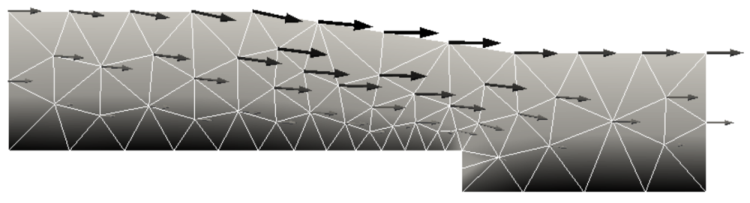
\includegraphics[width=\textwidth,angle=-5.7296]{stepflowlin}  % 0.1 radian = 5.7296 degrees
\caption{A 400 m thick glacier flowing over 100 m bedrock steps, with bed at angle $5.73^\circ$.  Arrows show velocity $\bu$ and shading is pressure $p$.}
% FIXME want steady surface too
\label{fig:stepflowlin}
\end{figure}


\section{Stokes equations}

Recall the Glen-Stokes model in equations (3), (4), (5) from the notes; the model is also described in \cite{GreveBlatter2009,JouvetRappaz2011}.  It applies on a 3D or 2D domain $\Omega$, according to the context, which must have a smooth-enough boundary to apply the boundary conditions but is otherwise general.  Allowing any Glen exponent $n\ge 1$, the equations are:
\begin{align}
\nabla \cdot \bu &= 0 &&\text{\emph{incompressibility}} \label{incompressible} \\
- \nabla \cdot \tau + \nabla p &= \rho \bg &&\text{\emph{stress balance}} \label{forcebalance} \\
D\bu &= A_n |\tau|^{n-1} \tau &&\text{\emph{Glen flow law}} \label{flowlaw}
\end{align}
The velocity $\bu$, pressure $p$, ice density $\rho$, acceleration of gravity $\bg$, deviatoric stress tensor $\tau$ and strain rate tensor $D\bu$ all appear.  Recall $D\bu$ involves derivatives of velocity:
\begin{equation}
(D\bu)_{ij} = \frac{1}{2} \left((u_i)_{x_j} + (u_j)_{x_i}\right) \label{strainrate}
\end{equation}

Though the notation here generally follows Table 1 in the notes, some usage is more general or flexible.  For example, the ice softness $A_n$ in \eqref{flowlaw} is now $n$-dependent.  Table 1 shows $A = A_3 = 10^{-16} \,\text{Pa}^{-3}\,\text{a}^{-1} = 3.1689 \times 10^{-24} \,\text{Pa}^{-3}\,\text{s}^{-1}$, but generally the units of $A_n$ are $\text{Pa}^{-n}\,\text{s}^{-1}$.  Regarding tensor norm notation we have:
\begin{align*}
|\tau|^2 = \frac{1}{2} \trace\left(\tau^2\right) = \frac{1}{2} \tau_{ij} \tau_{ij}, \qquad |D\bu|^2 = \frac{1}{2} \trace\left((D\bu)^2\right) = \frac{1}{2} (D\bu)_{ij} (D\bu)_{ij}
\end{align*}

Tensors $D\bu$ and $\tau$ are symmetric and have trace zero.  The full (Cauchy) stress tensor $\sigma$ is the deviatoric stress tensor $\tau$ minus the pressure,
\begin{equation}
    \sigma = \tau - p\,I,  \label{cauchystress}
\end{equation}
so equation \eqref{forcebalance} is simply $-\Div \sigma = \rho \bg$.  One may derive from \eqref{cauchystress} that $p = -\frac{1}{3} \trace(\sigma)$ in 3D, thus that the pressure is the negative of the average normal stress.  By definition $\Div\tau$ in \eqref{forcebalance} is a vector with components which are the divergences of the rows:
\begin{equation}
    \left(\nabla \cdot \tau\right)_i = \left(\tau_{i1}\right)_{x_1} + \left(\tau_{i2}\right)_{x_2} + \left(\tau_{i3}\right)_{x_3}  \label{divtaudefn}
\end{equation}
Thus $\nabla\cdot \tau$ is a column vector like $\nabla p$ and $\bg$ in \eqref{forcebalance}.

Recall the viscosity form of \eqref{flowlaw}, namely equation (15) in the notes:
\begin{equation}
\tau = 2\nu D\bu = B_n |D\bu|^{\frac{1}{n} - 1} D\bu  \label{viscflowlaw}
\end{equation}
Here $B_n = (A_n)^{-1/n}$ is the $n$-dependent ice hardness in units $\text{Pa}\,\text{s}^{1/n}$.  From \eqref{viscflowlaw} we can eliminate $\tau$ from equations \eqref{forcebalance}, \eqref{flowlaw} and rewrite them in terms of velocity and pressure only:
\begin{align}
\Div \bu &= 0 \label{incompagain} \\
- \nabla \cdot \left(B_n |D\bu|^{\frac{1}{n} - 1} D\bu\right) + \nabla p &= \rho \mathbf{g} \label{stokes}
\end{align}
The Stokes model is, from now on, equations \eqref{incompagain}, \eqref{stokes} with certain boundary conditions.  The solution is the velocity-pressure pair $(\bu,p)$.

Certain glacier-suitable boundary conditions are used in this document and in the code below.  To explain these, consider the numerical solution shown in Figure \ref{fig:stepflowlin}.  We assume that the base, top, inflow, and outflow boundary surfaces are all well-defined.  On the base we require no slip:
\begin{align}
\bu &= 0  &&\text{\emph{base}} \label{basebc} \\
\intertext{On the top we set a condition of zero applied stress, $\sigma\hbn=0$ or equivalently:}
\left(B_n |D\bu|^{\frac{1}{n} - 1} D\bu - pI\right) \hbn &= 0  &&\text{\emph{top}} \label{topbc} \\
\intertext{As shown in Figure \ref{fig:stepflowlin}, the left-side inflow boundary is a surface with outward normal $\hbn=\left<-1,0,0\right>^\top$ in all cases we solve.  On this surface we set a nonzero inflow velocity:}
\bu &= \left<f(z),0,0\right>^\top  &&\text{\emph{inflow}} \label{inflowbc} \\
\intertext{The inflow $f(z)$ will satisfy the slab-on-slope equations; see below.  On the outflow boundary, where $\hbn=\left<1,0,0\right>^\top$, $h$ is the surface elevation, and $g=|\bg|$, we set a nonzero hydrostatic normal stress and zero traction:}
\left(B_n |D\bu|^{\frac{1}{n} - 1} D\bu - pI\right) \hbn &= \left<-\rho g \cos\alpha (h-z),0,\rho g\sin\alpha (h-z)\right>^\top  &&\text{\emph{outflow}} \label{outflowbc}
\end{align}


\section{Slab-on-slope solutions}

Testing a numerical model requires verification tools, namely exact solutions.  Thus we recapitulate the construction of slab-on-slope solutions, as given in the notes, this time allowing any Glen exponent $n$.  We also determine the $n$-dependent ice hardness $B_n$ so that these solutions have the same surface velocity for any $n$, and we construct the outflow boundary condition used in more general situations.

Suppose the domain $\Omega$ is 2D, namely points $(x,y,z)$ where $y=0$.  Denote the components of velocity as $\bu=\left<u,v,w\right>$.  Suppose there is no variation in the cross-flow direction ($\partial/\partial y=0$) and no cross-flow velocity ($v=0$).  Also assume the force of gravity is downward but at angle $\alpha$ with the $z$-direction so $\bg = \left<g\sin\alpha,0,-g\cos\alpha\right>$ where $g=|\bg|$.  Equations \eqref{incompagain}, \eqref{stokes} now become the system
\begin{align}
u_x + w_z &= 0 \label{planeincomp} \\
- \left(B_n |D\bu|^{\frac{1}{n}-1} u_x\right)_x - \left(B_n |D\bu|^{\frac{1}{n}-1} \frac{1}{2} \left(u_z+w_x\right)\right)_z + p_x &= \rho g\sin\alpha \label{planestressx} \\
- \left(B_n |D\bu|^{\frac{1}{n}-1} \frac{1}{2} \left(u_z+w_x\right)\right)_x - \left(B_n |D\bu|^{\frac{1}{n}-1} w_z\right)_z + p_z &= -\rho g\cos\alpha \label{planestressz}
\end{align}
The strain-rate norm expands/simplifies to
\begin{equation}
    |D\bu| = \sqrt{\frac{1}{2} \left(u_x^2 + \frac{1}{2}(u_z+w_x)^2 + w_z^2\right)}  \label{planeDnorm}
\end{equation}
Equations \eqref{planeincomp}--\eqref{planeDnorm} are the 2D (strong) form of the Stokes model, written-out using coordinates $(x,z)$ and velocity $\bu=\left<u,w\right>$.

Now suppose there is no variation in $x$, i.e.~that $\partial/\partial_x=0$, and that the domain $\Omega$ is a slab such that $b < z < h$ for fixed ($x$-independent) values of the bed elevation $b$ and the surface elevation $h$.  This is the situation of an infinitely-long (or periodic) slab flow with $x$-independent boundary stresses (e.g.~no lubricated spots at the base).  Then the system simplifies to $w_z=0$ and
\begin{equation}
- \left(B_n |D\bu|^{\frac{1}{n}-1} \frac{1}{2} u_z\right)_z = \rho g\sin\alpha, \quad
- \left(B_n |D\bu|^{\frac{1}{n}-1} w_z\right)_z + p_z = -\rho g\cos\alpha \label{slabstresses}
\end{equation}
The strain-rate norm simplifies to $|D\bu| = \sqrt{\frac{1}{2} \left(\frac{1}{2}u_z^2 + w_z^2\right)}$.

If we further assume that there is no slip at the base then $w=0$ identically.  Then the second of equations \eqref{slabstresses} allows integration with respect to $z$ yielding a formula for $p$.  Assuming zero pressure at the surface gives the hydrostatic pressure profile
\begin{equation}
p(z) = \rho g\cos\alpha (h-z)  \label{pslab}
\end{equation}
Also $|D\bu| = \frac{1}{2} |u_z|$.  From \eqref{slabstresses} we now have a single nontrivial equation to solve for the horizontal velocity:
    $$- \left(\frac{B_n}{2^{\gamma+1}} |u_z|^\gamma u_z\right)_z = \rho g\sin\alpha$$
The flow of a viscous, non-sliding fluid on a uniform slab will be such that $u_z>0$, so, with rearrangement, the equation is now
    $$\left((u_z)^{1/n} \right)_z = - \frac{2^{1/n} \rho g\sin\alpha}{B_n}$$
Again this can be integrated from the surface $z=h$, using the no-stress (no traction) condition, which simplifies to $u_z=0$, to give
\begin{equation}
u_z = 2 \left(\frac{\rho g\sin\alpha}{B_n}\right)^n (h-z)^n  \label{uzslab}
\end{equation}
Integrating vertically one more time, from the base $z=b$ where $u=0$, gives
\begin{equation}
u(z) = \frac{2}{n+1} \left(\frac{\rho g\sin\alpha}{B_n}\right)^n \left((h-b)^{n+1} - (h-z)^{n+1}\right)  \label{uslab}
\end{equation}

Suppose we want comparable solutions, with glaciologically-reasonable ice velocities, for any $n\ge 1$.  Ice sheet modeling tradition \cite{GreveBlatter2009}, and glaciological experiments starting with Glen, suggest we base our work on $n=3$.  From the ice softness value $A_3 = 3.1689 \times 10^{-24} \,\text{Pa}^{-3}\,\text{s}^{-1}$ we get $B_3 = (A_3)^{-1/3} = 6.8082\times 10^7\,\text{Pa}\,\text{s}^{1/3}$.  We now compute $B_n$ for any $n\ge 1$ such the slab-on-slope surface velocity $u(h)$ from \eqref{uslab} matches the value in the $n=3$ case.  The result is
\begin{equation}
B_n = \left(\frac{4}{n+1}\right)^{1/n} \Big(\rho g \sin\alpha (h-b)\Big)^{(n-3)/n} {B_3\,}^{3/n}  \label{Bnfromsurface}
\end{equation}
For example, suppose $h-b=400$ m and $\alpha=0.1$ radians (about $5.7$ degrees).  Using $B_n$ from \eqref{Bnfromsurface} gives a surface velocity of $u(h)=906.092 \,\text{m}\,\text{a}^{-1}$ from \eqref{uslab} independent of $n\ge 1$.  For some glaciologically-relevant end-cases $n=1,4$ \cite{GreveBlatter2009}, the result from \eqref{Bnfromsurface} is $B_1=4.9663\times 10^{12}\,\text{Pa}\,\text{s}$ and $B_4=1.7320\times 10^{7}\,\text{Pa}\,\text{s}^{1/4}$.  The Newtonian viscosity $\nu=B_1/2$ is about $10^{16}$ times more viscous than liquid water but about $10^7$ times less viscous than granite (both at $25^\circ \,\text{C}$, and according to wikipedia).

Formulas \eqref{pslab} and \eqref{uslab} will be used for verifying the numerical solver.  Additionally they allow us to set boundary conditions which lead to glaciologically-reasonable solutions even when modeling a small part of a glacier.  Specifically we do this for the geometry shown in Figure \ref{fig:stepflowlin}.  The inflow side of the region has \eqref{uslab} applied as a Dirichlet condition, i.e.~equation \eqref{inflowbc}.  Also, the outflow side has a normal stress computed from the slab-on-slope solution.  From \eqref{uzslab} above, and the facts that $w=0$, $u_x=0$, and $|D\bu| = \frac{1}{2} u_z$, we find that because $\hbn=\left<1,0\right>$ is the outward normal on the outflow side,
\begin{align*}
\sigma \hbn &= \left(B_n |D\bu|^{\frac{1}{n}-1} D\bu - pI\right)\hbn = \left(B_n |D\bu|^{\frac{1}{n}-1} \begin{pmatrix} u_x & \frac{1}{2}(u_z+w_x) \\ \frac{1}{2}(u_z+w_x) & w_z \end{pmatrix} - pI\right)\hbn \\
    &= B_n \left(\frac{1}{2} u_z\right)^{\frac{1}{n}-1} \begin{pmatrix} 0 \\ \frac{1}{2} u_z \end{pmatrix} - \begin{pmatrix} p \\ 0 \end{pmatrix} = \begin{pmatrix} - p \\ \frac{B_n}{2^{1/n}} (u_z)^{1/n} \end{pmatrix} = \begin{pmatrix} - \rho g\cos\alpha (h-z) \\ \rho g\sin\alpha (h-z) \end{pmatrix}
\end{align*}
This justifies formula \eqref{outflowbc}.


\section{Weak form}

The Stokes equations \eqref{incompagain}, \eqref{stokes} are PDEs called the \emph{strong form} of the model.  The \emph{weak form}, needed to construct an FE method \cite{Elmanetal2014}, is derived by multiplying the equations by arbitrary test functions and then integrating over $\Omega$ so as to define a scalar-valued nonlinear functional $F$.  In the FE method the test functions will be locally constructed from the triangular mesh.

The solution is the pair $(\bu,p)$ where $\bu\in V_D$ and $p \in Q$ for function spaces precisely identified in \cite{JouvetRappaz2011}.  The test functions come from nearly the same spaces, with differences relating (only) to the value of Dirichlet boundary conditions: the solution velocity $\bu\in V_D$ satisfies \eqref{basebc}, \eqref{inflowbc} while the test functions $\bv\in V_0$ are zero on both base and inflow surfaces.  The test pressures are from $Q$ just like $p$.

We multiply \eqref{incompagain} by $q\in Q$ and \eqref{stokes} by $\bv\in V_0$, and add and integrate to define $F$:
\begin{equation}
F(\bu,p;\bv,q) = \int_\Omega - \left(\nabla \cdot \left(B_n |D\bu|^{\frac{1}{n} - 1} D\bu\right)\right)\cdot \bv + \nabla p \cdot \bv - \rho \mathbf{g} \cdot \bv - \left(\nabla \cdot \bu\right) q \label{nonfuncone}
\end{equation}
This functional must be zero at the solution $(\bu,p)$ in the sense that $F(\bu,p;\bv,q) = 0$ for all  $\bv\in V_0$ and $q\in Q$.  Next, integration-by-parts rewrites $F$ to balance the number of derivatives on $(\bv,q)$ and $(\bu,p)$.  Recall the product rule $\nabla \cdot(f\bX) = \grad f\cdot \bX + f \nabla \cdot \bX$ and the divergence theorem $\int_\Omega \nabla \cdot \bX = \int_{\partial \Omega} \bX \cdot \hbn$.  Again denoting $\tau = B_n |D\bu|^{\frac{1}{n} - 1} D\bu$, from these rules we have
\begin{align*}
\int_\Omega \left(\nabla \cdot \tau\right)\cdot \bv &= \sum_{j=1}^3 \int_\Omega \nabla \cdot (\tau_{j\circ})\, v_j = \sum_{j=1}^3 \int_\Omega \nabla \cdot (\tau_{j\circ} v_j) - \tau_{j\circ} \nabla v_j \\
  &= \sum_{j=1}^3 \int_{\partial \Omega} (\tau_{j\circ} v_j) \cdot \hbn - \int_\Omega \tau_{j\circ} \cdot \nabla v_j = \int_{\partial \Omega} (\tau \hbn)\cdot \bv - \int_\Omega \trace(\tau \nabla \bv)
\end{align*}
where $\circ$ denotes an index which is iterated-over and $\tau_{j\circ}$ denotes the $j$th row of $\tau$.  Here $\grad\bv$ defines a $3\times 3$ matrix,
\newcommand{\trefthree}[3]{\left[\begin{array}{c|c|c} & & \\ #1 & #2 & #3 \\ & & \end{array}\right]}
    $$\grad \bv = \trefthree{\grad v_1}{\grad v_2}{\grad v_3} = \begin{bmatrix}
    (v_1)_{x_1} & (v_2)_{x_1} & (v_3)_{x_1} \\
    (v_1)_{x_2} & (v_2)_{x_2} & (v_3)_{x_2} \\
    (v_1)_{x_3} & (v_2)_{x_3} & (v_3)_{x_3}
    \end{bmatrix}$$
so
    $$\trace(\tau \grad \bv) = \sum_{j=1}^3 \tau_{j\circ} \cdot \grad v_j = \sum_{i,j=1}^3 \tau_{ji} (v_j)_{x_i}$$
Also, because $\trace(AB)=0$ if $A$ is symmetric and $B$ is antisymmetric, in fact $\trace(\tau \grad \bv) = \trace(\tau D\bv)$.  (To show this take $A=\tau$ and $B=\grad\bv-D\bv$.  Note that many sources write $A:B$ for $\trace(AB)$.)

In addition we do a straightforward integration-by-parts on the pressure portion of $F$:
    $$\int_\Omega \nabla p \cdot \bv = \int_\Omega \nabla\cdot (p\,\bv) - p (\nabla \cdot \bv) = \int_{\partial \Omega} p\hbn \cdot \bv - \int_\Omega p (\nabla \cdot \bv)$$
These facts, plus denoting $\sigma=\tau-pI$ for clarity, allow us to rewrite \eqref{nonfuncone} with an integral of the normal stress over the boundary:
\begin{equation}
F(\bu,p;\bv,q) = -\int_{\partial\Omega} (\sigma \hbn)\cdot \bv + \int_\Omega \trace(\tau D\bv) - p (\nabla \cdot \bv) - \left(\nabla \cdot \bu\right) q - \rho \mathbf{g} \cdot \bv \label{nonfunctwo}
\end{equation}
Now $\bu,\bv$ appear with at most first derivatives and $p,q$ appear without derivatives.

Recall that $\bv\in V_0$ satisfies $\bv=0$ along the base and inflow surfaces so these portions of the above integral over $\partial\Omega$ are zero.  Conditions \eqref{topbc}, \eqref{outflowbc} therefore completely eliminate the unknown solution $\bu,p$ from the boundary integral.  This yields our final formula for the nonlinear functional:
\begin{align}
F(\bu,p;\bv,q) &= \int_\Omega B_n |D\bu|^{\frac{1}{n} - 1} \trace(D\bu D\bv) - p (\nabla \cdot \bv) - \left(\nabla \cdot \bu\right) q \label{defineF} \\
    &\qquad  - \int_\Omega \rho \mathbf{g} \cdot \bv - \int_{\{\text{outflow}\}} \rho g (h-z) v_1  \notag
\end{align}
The last two integrals can be regarded as the source terms.  For example, if we replace them by zero---no gravity or outflow stress---then we expect solution $\bu=0$ and $p=0$.

The weak formulation of the Stokes model is the statement that $F$ is zero in all directions at the solution: the solution $\bu\in V_D$ and $p\in Q$ satisfies
\begin{equation}
F(\bu,p;\bv,q) = 0 \qquad \text{ for all } \bv\in V_0 \text{ and } q\in Q  \label{weak}
\end{equation}
This weak formulation is proven in \cite{JouvetRappaz2011} to be well-posed under reasonable assumptions about the domain $\Omega$ and boundary data.  These assumptions will be satisfied in the cases we consider.  Thus there is exactly one solution pair $(\bu,p)$.  From now on our goal is to approximate this solution numerically.


\section{Finite element method}

FIXME

\section{Surface kinematical equation, and moving the mesh}

A real glacier changes shape as it flows.  We want our model to do that too.  Form now on we regard the domain on which the Stokes equations apply as the time-dependent set
\begin{equation}
\Omega_t = \left\{(x,z)\,\big|\, b(x) \le z \le h(x,t)\right\}  \label{Omegat}
\end{equation}
where $z=b(x)$ is the bedrock elevation and $z=h(x,t)$ is the time-dependent ice surface elevation.  At any time $t$ the Stokes equations, as already covered, apply on $\Omega_t$.

\section{Firedrake code}

FIXME: show block figure with blocks = (gendomain.py,gmsh,flow.py,paraview) and file formats as arrows (.geo,.msh,.pvd)

FIXME: show codes here

%\VerbatimInput[frame=lines,numbers=left,stepnumber=5,fontsize=\footnotesize]{../genstepmesh.py}

%\VerbatimInput[frame=lines,numbers=left,stepnumber=5,fontsize=\footnotesize]{../flowstep.py}

\footnotesize

\bigskip
%from: \bibliographystyle{siam}

\begin{thebibliography}{3}

%\bibitem{BaliseRaymond1985}
%{\sc M.~Balise and C.~Raymond}, {\em Transfer of basal sliding variations to
%  the surface of a linearly-viscous glacier}, J. Glaciol., 31 (1985),
%  pp.~308--318.

%\bibitem{Brownetal2013}
%{\sc J.~Brown, B.~Smith, and A.~Ahmadia}, {\em Achieving textbook multigrid
%  efficiency for hydrostatic ice sheet flow}, SIAM J. Sci. Computing,
%  35 (2013), pp.~B359--B375.

\bibitem{Elmanetal2014}
{\sc H.~C. Elman and D.~J. Silvester and A.~J. Wathen}, {\em Finite Elements
  and Fast Iterative Solvers: with Applications in Incompressible Fluid Dynamics},
  Oxford University Press, 2nd~ed., 2014.

\bibitem{GreveBlatter2009}
{\sc R.~Greve and H.~Blatter}, {\em Dynamics of {I}ce {S}heets and {G}laciers},
  Advances in Geophysical and Environmental Mechanics and Mathematics,
  Springer, 2009.

\bibitem{JouvetRappaz2011}
{\sc G.~Jouvet and J.~Rappaz}, {\em Analysis and finite element approximation
  of a nonlinear stationary {S}tokes problem arising in glaciology}, Advances
  in Numerical Analysis, (2011).

%\bibitem{Lengetal2012}
%{\sc W.~Leng, L.~Ju, M.~Gunzburger, S.~Price, and T.~Ringler}, {\em A parallel
%  high-order accurate finite element nonlinear {S}tokes ice sheet model and
%  benchmark experiments}, J. Geophys. Res., 117 (2012).

\end{thebibliography}


\end{document}
